%% beamer/knitr slides 
%% for Statistical Modeling and Data Visualization course @ UMass
%% Nicholas Reich: nick [at] schoolph.umass.edu


\documentclass[table]{beamer}\usepackage[]{graphicx}\usepackage[]{color}
%% maxwidth is the original width if it is less than linewidth
%% otherwise use linewidth (to make sure the graphics do not exceed the margin)
\makeatletter
\def\maxwidth{ %
  \ifdim\Gin@nat@width>\linewidth
    \linewidth
  \else
    \Gin@nat@width
  \fi
}
\makeatother

\definecolor{fgcolor}{rgb}{0.345, 0.345, 0.345}
\newcommand{\hlnum}[1]{\textcolor[rgb]{0.686,0.059,0.569}{#1}}%
\newcommand{\hlstr}[1]{\textcolor[rgb]{0.192,0.494,0.8}{#1}}%
\newcommand{\hlcom}[1]{\textcolor[rgb]{0.678,0.584,0.686}{\textit{#1}}}%
\newcommand{\hlopt}[1]{\textcolor[rgb]{0,0,0}{#1}}%
\newcommand{\hlstd}[1]{\textcolor[rgb]{0.345,0.345,0.345}{#1}}%
\newcommand{\hlkwa}[1]{\textcolor[rgb]{0.161,0.373,0.58}{\textbf{#1}}}%
\newcommand{\hlkwb}[1]{\textcolor[rgb]{0.69,0.353,0.396}{#1}}%
\newcommand{\hlkwc}[1]{\textcolor[rgb]{0.333,0.667,0.333}{#1}}%
\newcommand{\hlkwd}[1]{\textcolor[rgb]{0.737,0.353,0.396}{\textbf{#1}}}%
\let\hlipl\hlkwb

\usepackage{framed}
\makeatletter
\newenvironment{kframe}{%
 \def\at@end@of@kframe{}%
 \ifinner\ifhmode%
  \def\at@end@of@kframe{\end{minipage}}%
  \begin{minipage}{\columnwidth}%
 \fi\fi%
 \def\FrameCommand##1{\hskip\@totalleftmargin \hskip-\fboxsep
 \colorbox{shadecolor}{##1}\hskip-\fboxsep
     % There is no \\@totalrightmargin, so:
     \hskip-\linewidth \hskip-\@totalleftmargin \hskip\columnwidth}%
 \MakeFramed {\advance\hsize-\width
   \@totalleftmargin\z@ \linewidth\hsize
   \@setminipage}}%
 {\par\unskip\endMakeFramed%
 \at@end@of@kframe}
\makeatother

\definecolor{shadecolor}{rgb}{.97, .97, .97}
\definecolor{messagecolor}{rgb}{0, 0, 0}
\definecolor{warningcolor}{rgb}{1, 0, 1}
\definecolor{errorcolor}{rgb}{1, 0, 0}
\newenvironment{knitrout}{}{} % an empty environment to be redefined in TeX

\usepackage{alltt}


%       ************************************************
%       **        LaTeX preamble to be used with all 
%	**        statsTeachR labs/handouts.
%
%	Author: Nicholas G Reich
%	Last modified: 14 January 2014
%	************************************************

% \documentclass[table]{beamer}

%	Set theme (a nice plain one)
\usetheme{Malmoe}

%	Use named colors, set main color of theme
%		to match Web site color:
\definecolor{MainColor}{RGB}{10, 74, 109}
\colorlet{MainColorMedium}{MainColor!50}
\colorlet{MainColorLight}{MainColor!20}
\usecolortheme[named=MainColor]{structure} 

%	For tables
%[dvipsnames] [table]
\usepackage{xcolor}

%% calling tabu.sty, assuming a particular directory structure
\usepackage{../../slide-includes/tabu}	% Even fancier than tabulary
\usepackage{multirow}

%	Just for the degree symbol
\usepackage{textcomp}

%	Get rid of footline (page, author, etc. on each slide)
\setbeamertemplate{footline}{}
%	Get rid of navigation buttons
\setbeamertemplate{navigation symbols}{}

%	Make footnotes not ugly
\usepackage{hanging}
\setbeamertemplate{footnote}{\raggedright\hangpara{1em}{1}\makebox[1em][l]{\insertfootnotemark}\footnotesize\insertfootnotetext\par}

%	Text style for code snippets inline in text:
\newcommand{\codeInline}[1]{\texttt{#1}}

%	Text style for emphasis stronger than \emph:
%		(Note, this doesn't toggle the way \emph does.
%			(Note, this can be done, didn't seem worth the trouble.))
\newcommand{\strong}[1]{{\bfseries{#1}}}


%        ******	Define title page	**********************
\setbeamertemplate{title page}{
	{\color{MainColor}
	% There must be a better way than this -vspace at
	%	 the top and bottom of the page to reduce the 
	%	 bottom margin, but I can't find one that works.
	\vspace{-6em}

% 	% Go to a lot of trouble to get the title in a
% 	%	nice box, since customizing a beamer block
% 	%	does not entirely work here (I don't know why)
	\newlength{\titleBoxWidth}
	\setlength{\titleBoxWidth}{\textwidth}
	\addtolength{\titleBoxWidth}{-2.0em}
	\setlength{\fboxsep}{1.0em}
	\setlength{\fboxrule}{0pt}
	\fcolorbox{MainColor!25}{MainColor!25}{
		\parbox{\titleBoxWidth}{
			\raggedright
			\LARGE\textbf{\inserttitle}
		}	% end parbox
	}	% end fcolorbox

	\vfill
	\small{Author: \insertauthor}
	\vspace{\baselineskip}

	\small{\Course}

	\small{\Instructor}
	\vspace{\baselineskip}

	%\small{\emph{This material is part of the \strong{statsTeachR} project}}

	\vspace{0.33\baselineskip}\scriptsize{\emph{\LicenseText}}


		\vspace{-15em}

	}	% end color
	\clearpage
}	% end define title page

%	The following variables are assumed by the standard preamble:
%	Global variable containing module name:
\title{Introduction to \\ Telling Stories with Data}
%	Global variable containing module shortname:
%		(Currently unused, may be used in future.)
% \newcommand{\ModuleShortname}{introRegression}
%	Global variable containing author name:
\author{Nicholas G Reich}
%	Global variable containing text of license terms:
\newcommand{\LicenseText}{Slides available under the Creative Commons Attribution-ShareAlike 3.0 Unported License: http://creativecommons.org/licenses/by-sa/3.0/deed.en\textunderscore US }
%	Instructor: optional, can leave blank.
%		Recommended format: {Instructor: Jane Doe}
\newcommand{\Instructor}{}
%	Course: optional, can leave blank.
%		Recommended format: {Course: Biostatistics 101}
\newcommand{\Course}{}


\input{../../slide-includes/shortcuts}

\hypersetup{colorlinks,linkcolor=,urlcolor=MainColor}


%	******	Document body begins here	**********************
\IfFileExists{upquote.sty}{\usepackage{upquote}}{}
\begin{document}

%	Title page
\begin{frame}[plain]
	\titlepage
\end{frame}

%	******	Everything through the above line must be placed at
%		the top of any TeX file using the statsTeachR standard
%		beamer preamble. 



%%%%%%%%%%%%%%%%%%%%%%%%%%%%%%%%%%%%%%%%%%


\begin{frame}{What are data?}


\vspace{1em}

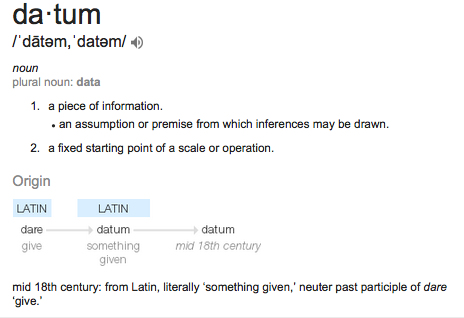
\includegraphics[width=.5\textwidth]{figure-static/data-definition.png}
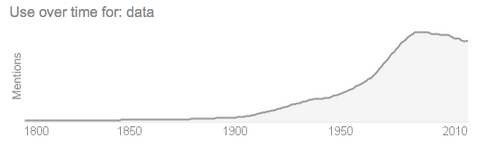
\includegraphics[width=.5\textwidth]{figure-static/data-usage-over-time.png}


\begin{block}{Data as building blocks}

\begin{itemize}
	\item Data are units of information, encoded for processing, e.g. ``machine-readable''
	\item Data, like words, can be woven together to create new conceptual understanding
	\item Data are the raw material of the digital economy.
\end{itemize}

\end{block}


\end{frame}


\begin{frame}{What are models? (see Kaplan, Chapter 1)}


\begin{block}{A (simplified) representation of a system of inter-relationships.}

\begin{itemize}
	\item Models can be mathematical, physical, mental, visual, etc...
	\item In representing the world, models attempt to create an accurate representation of some aspect of reality, ideally based on data.
	\item Classic quote: "all models are wrong, some are useful."
\end{itemize}

\end{block}

Mathematically, we can think of models like functions
$$ y = f(x_1, x_2, ...) + error $$



\end{frame}



\begin{frame}{Communicating ideas with evidence}

\begin{block}{What is a narrative? [From the OED]}

\em An account of a series of events, facts, etc., given in order and with the establishing of connections between them; a narration, a story, an account.

\em 
\begin{itemize}
  \item A data-driven narrative communicates the results of a model.
  \item Important to let the data lead our belief, not the other way around!!
\end{itemize}

\end{block}

\bigskip

\begin{block}{Telling stories with data}

\begin{itemize}
	\item raw material: words, data
	\item tools: code, software, computers, statistical models
	\item finished product: visualization, explanations, inference
\end{itemize}

\end{block}


\end{frame}


%%%%%%%%%%%%%%%%%%%%%%%%%%%%%%%%%%%%%%%%%%

%\begin{frame}
%
%\begin{centering}
%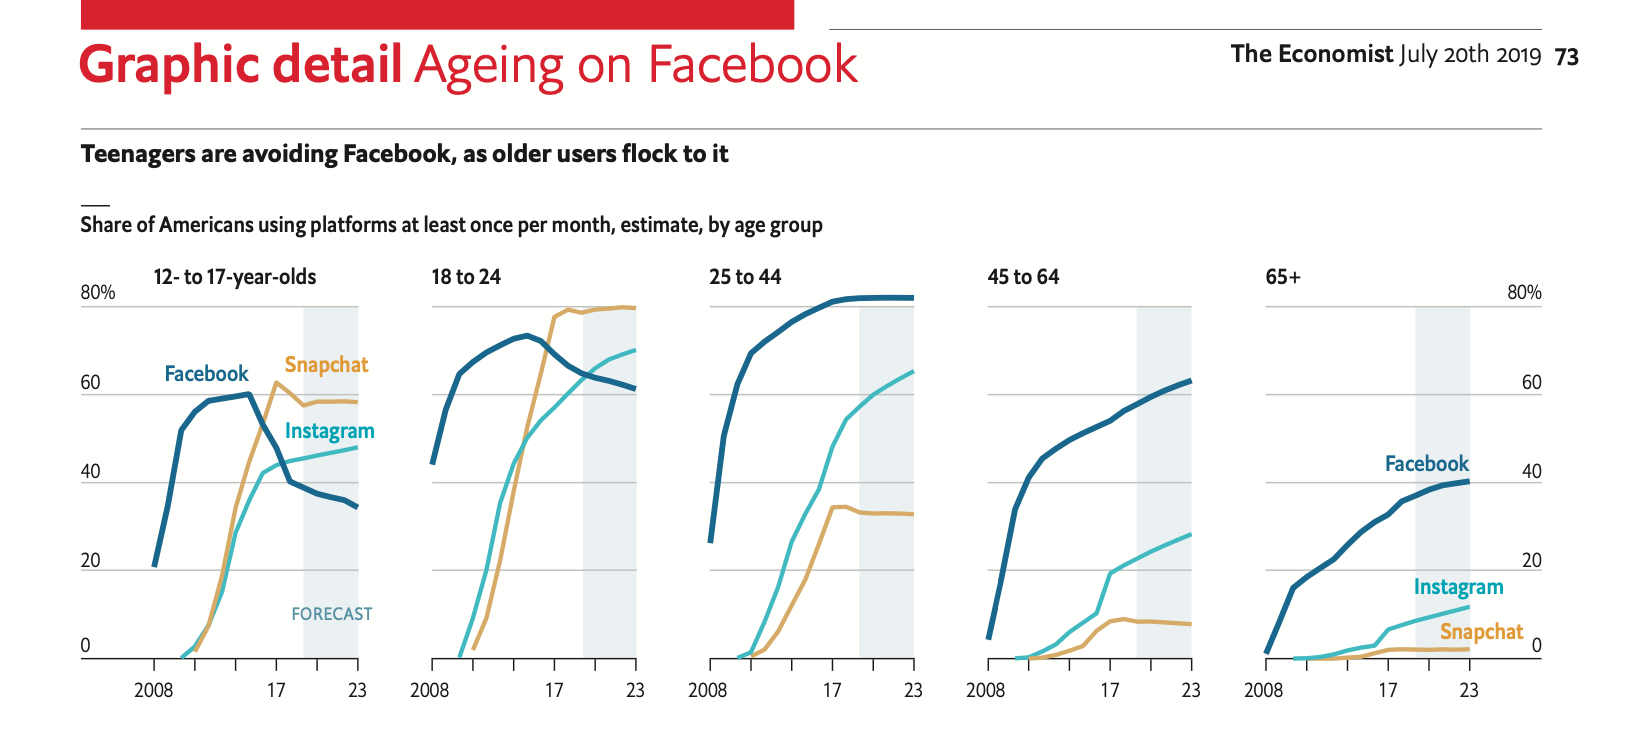
\includegraphics[width=\textwidth]{figure-static/graphic-detail-ageing-facebook.png}
%
%\end{centering}
%
%\end{frame}

%%%%%%%%%%%%%%%%%%%%%%%%%%%%%%%%%%%%%%%%%%


\begin{frame}

\centering 


\includegraphics[width=\textwidth]{figure-static/538-women-of-color-banner.png}

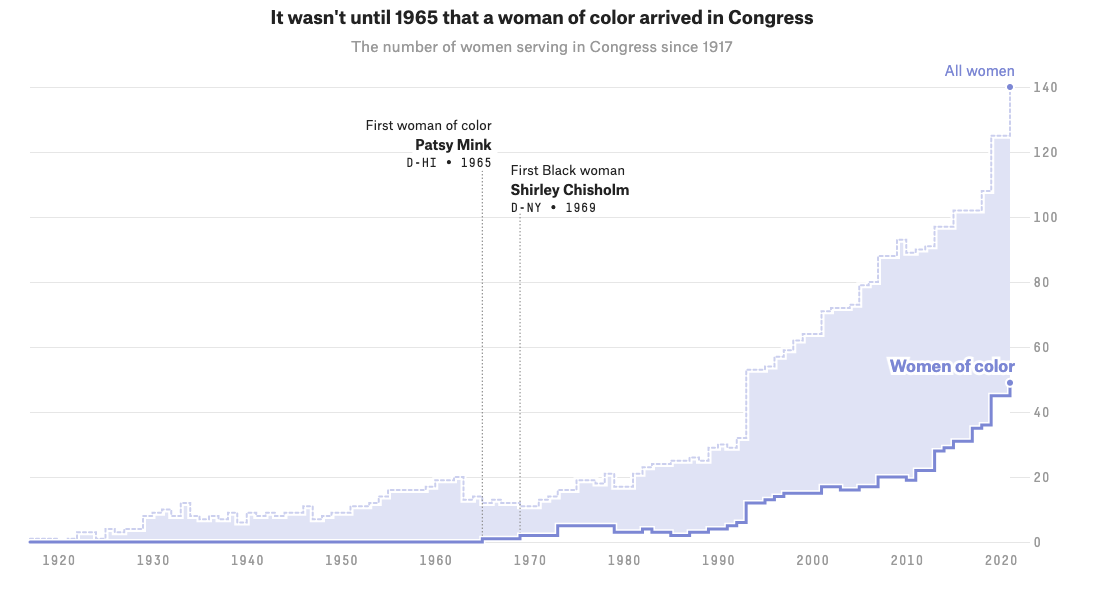
\includegraphics[width=\textwidth]{figure-static/538-women-of-color-timeline.png}

\tiny \url{https://projects.fivethirtyeight.com/women-of-color-congress-2020/}

\end{frame}




%%%%%%%%%%%%%%%%%%%%%%%%%%%%%%%%%%%%%%%%%%


\begin{frame}

\centering

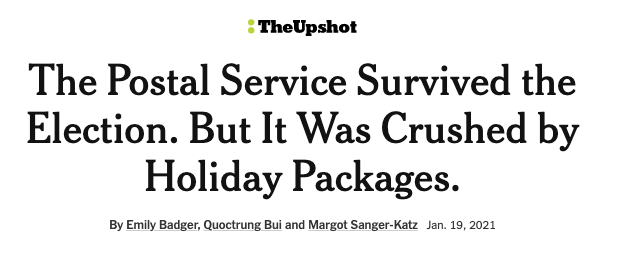
\includegraphics[width=.6\textwidth]{figure-static/upshot-postal-banner.png}

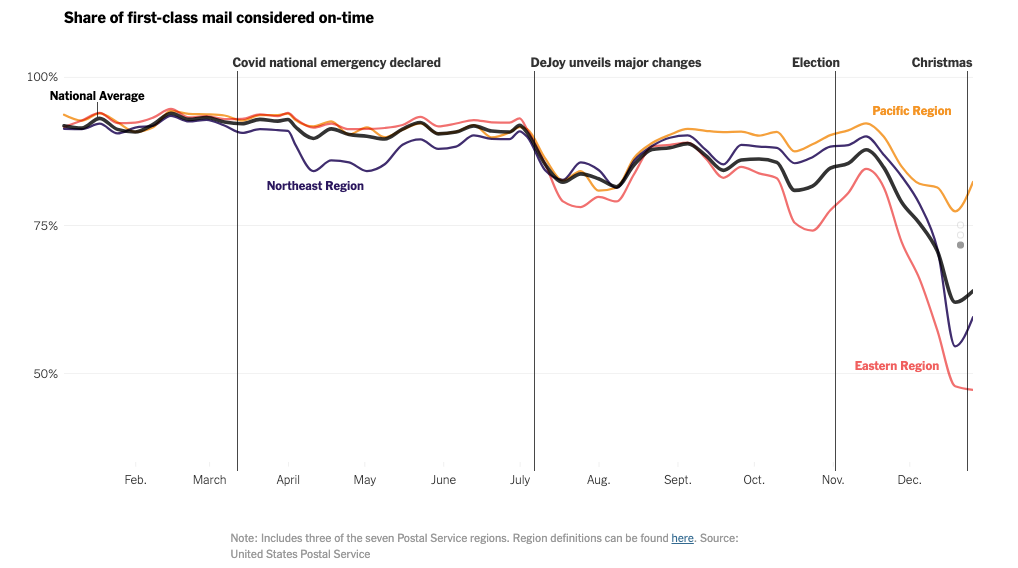
\includegraphics[width=.9\textwidth]{figure-static/upshot-postal-timeseries.png}

\tiny \url{https://www.nytimes.com/interactive/2021/01/19/upshot/postal-service-survived-election-but-crushed-by-holidays.html}

\end{frame}


%%%%%%%%%%%%%%%%%%%%%%%%%%%%%%%%%%%%%%%%%%

\begin{frame}

\centering 

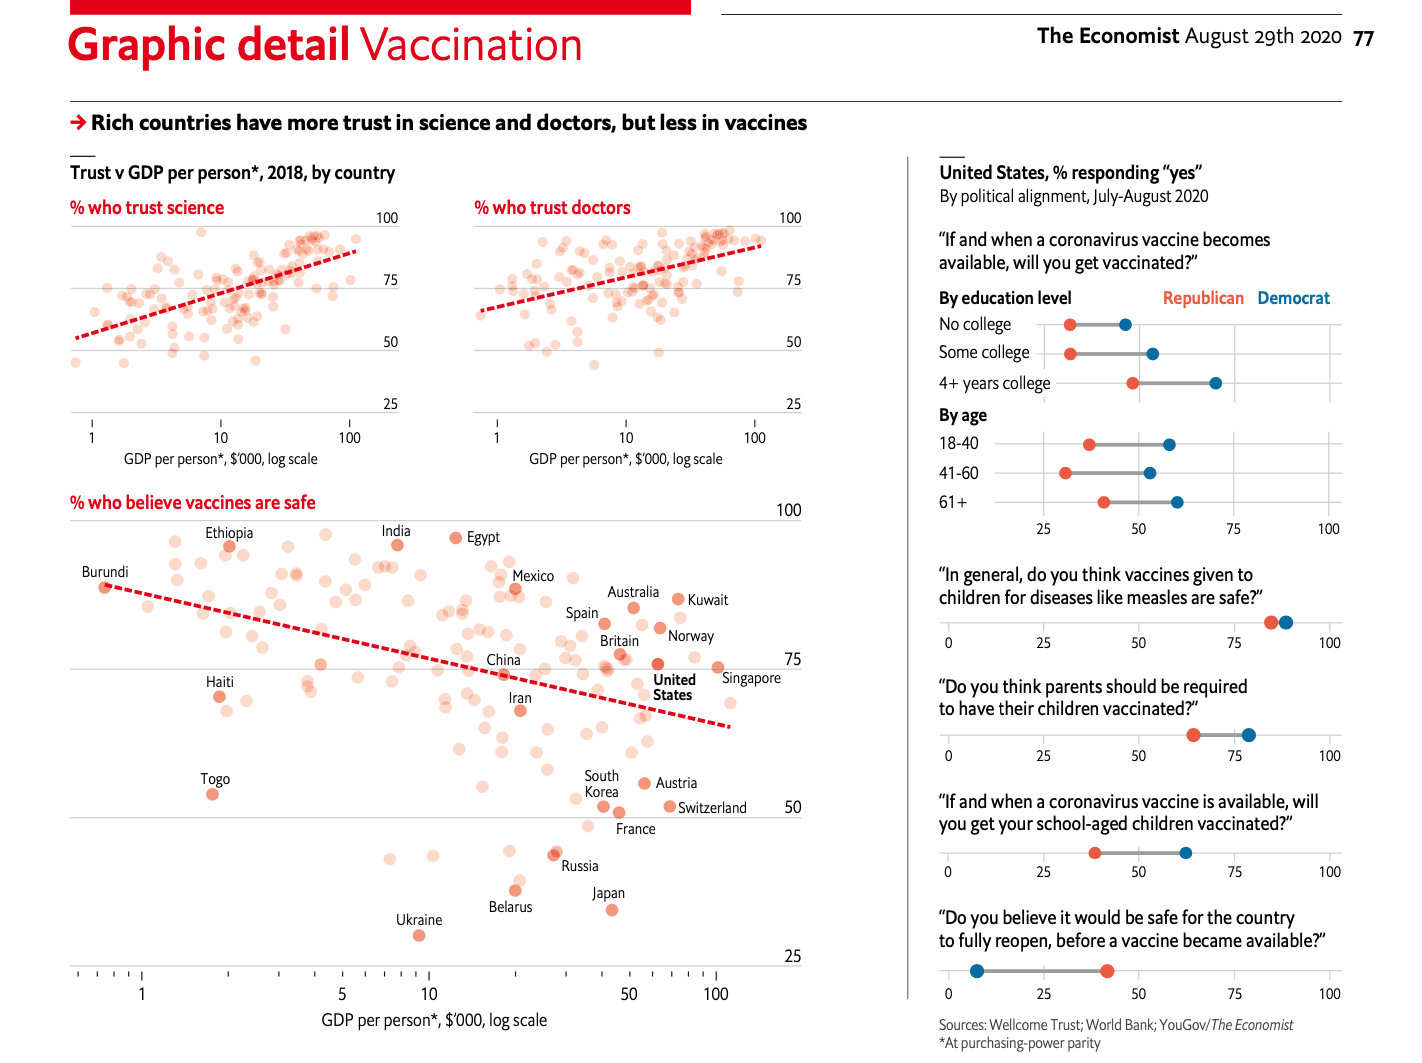
\includegraphics[width=\textwidth]{figure-static/graphic-detail-vaccination.png}

\tiny \url{https://www.economist.com/graphic-detail/2020/08/29/conspiracy-theories-about-covid-19-vaccines-may-prevent-herd-immunity}

\end{frame}

%%%%%%%%%%%%%%%%%%%%%%%%%%%%%%%%%%%%%%%%%%


\begin{frame}{How to tell a story using data}
Telling stories with data requires
\begin{itemize}
    \item a topic for the story you want to tell
    \item detective work
    \item creativity, both scientific and artistic
    \item experimentation with different storylines
    \item statistical literacy
    \item good data (good data does not necessarily equal ``big data'')
\end{itemize}

\end{frame}

%%%%%%%%%%%%%%%%%%%%%%%%%%%%%%%%%%%%%%%%%%


\begin{frame}{Common mistakes in data storytelling}

\begin{itemize}
    \item not knowing the audience
    \item making the story too complex too quickly
    \item trying to make it too complicated
    \item encouraging correlation to be seen as causation
    \item missing the little things (clear axis labels, plot annnotations)
\end{itemize}

\end{frame}


%%%%%%%%%%%%%%%%%%%%%%%%%%%%%%%%%%%%%%%%%%


\begin{frame}{A process for data analysis}

\includegraphics[width=\textwidth]{../../slide-includes/data-science-program.png}

\bigskip

This is where we are going to spend most of our time this semester. With a bit of a focus on public health applications. 

\bigskip

 \tiny Figure credits: \url{https://r4ds.had.co.nz/introduction.html}

\end{frame}


\end{document}
